\section{The Same Model Quantity on Both Axes}
\label{app:same-predictor}

In the main analysis, brain similarity is computed from the model's contextual embeddings and behavioral similarity from its surprisal. The trade-off could therefore reflect what each quantity captures rather than a difference between the two human targets. We repeat the analysis with one quantity on both axes: the whole-network embedding RDM for behavior as well (Figure~\ref{fig:sameq-pareto}A, Table~\ref{tab:rsa-sameq}, left), and the $|\Delta$surprisal$|$ RDM for the brain as well (Figure~\ref{fig:sameq-pareto}B, Table~\ref{tab:rsa-sameq}, right). Everything else is as in Section~\ref{sec:results-all}: same models, datasets, confounds, splits and references, and the same matched-scale regression.

\begin{figure}[h]
\centering
\begin{minipage}[t]{.49\linewidth}\textbf{A}\par\centering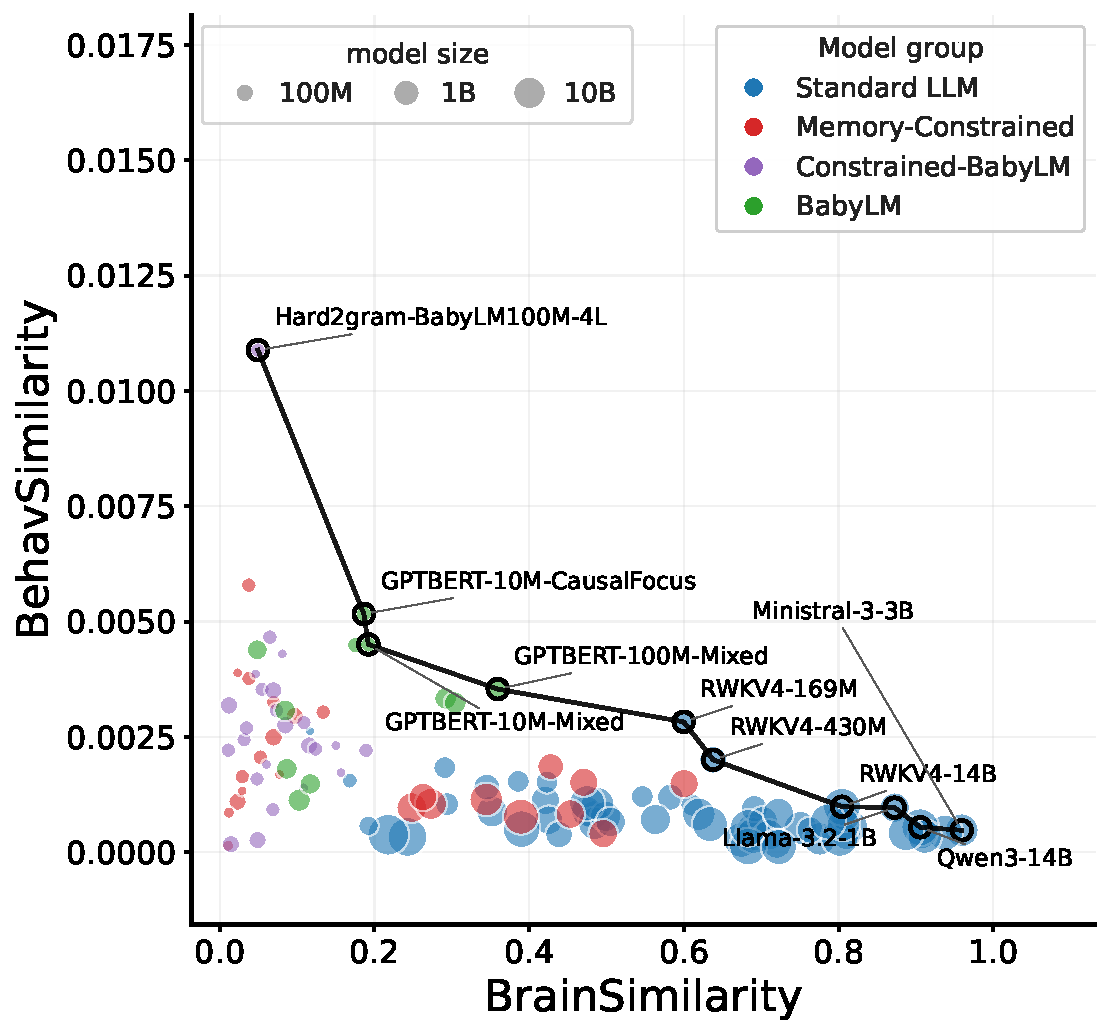
\includegraphics[width=\linewidth]{figures/rsa_embboth_pareto.pdf}\end{minipage}\hfill
\begin{minipage}[t]{.49\linewidth}\textbf{B}\par\centering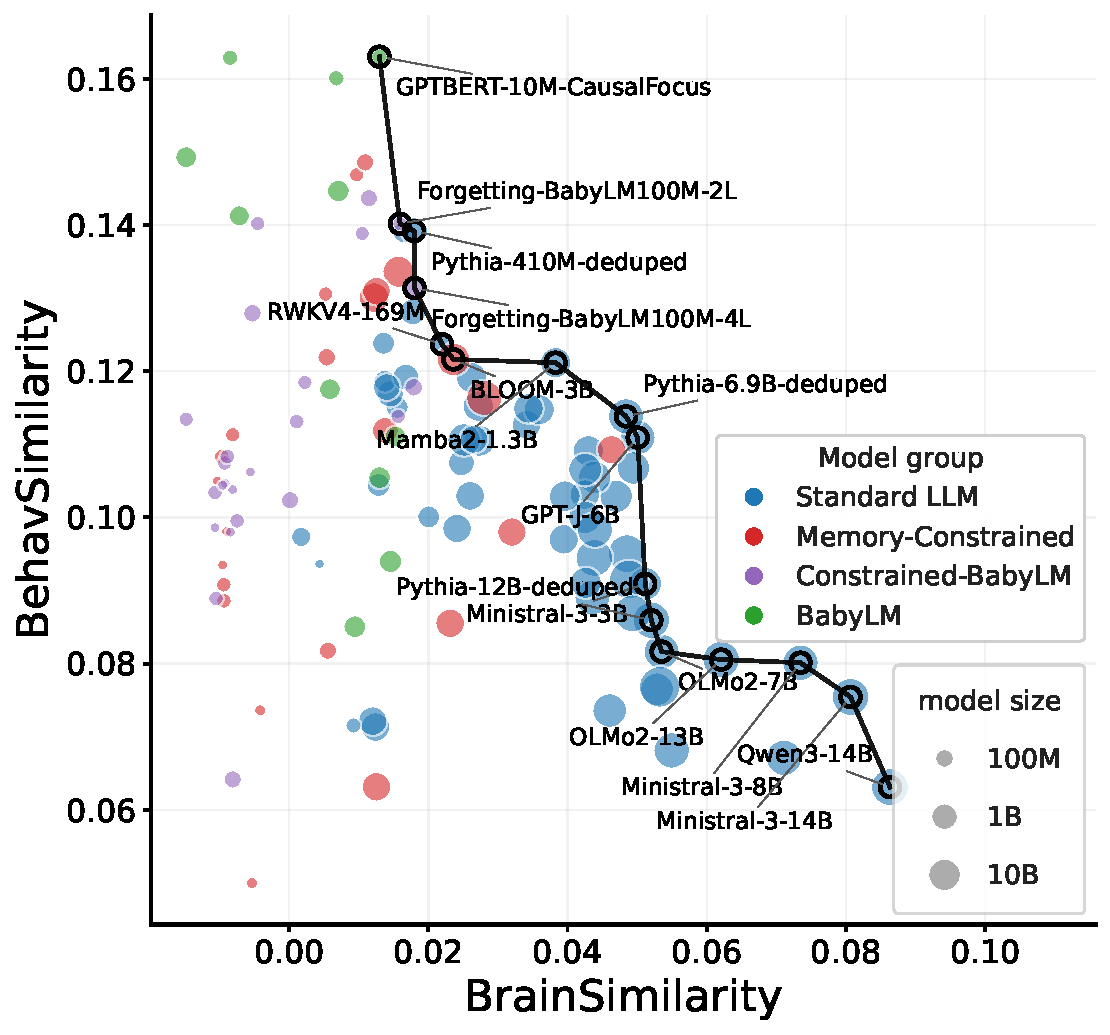
\includegraphics[width=\linewidth]{figures/rsa_surpboth_pareto.pdf}\end{minipage}
\caption{Brain similarity against behavioral similarity with the same model quantity on both axes (118 models). (A) Whole-network embedding RDM on both axes: brain similarity as in Figure~\ref{fig:method}B; behavioral similarity is the median over the 16 reading measures of the embedding-RDM score divided by the measure's split-half reference. (B) $|\Delta$surprisal$|$ RDM on both axes: behavioral similarity as in Figure~\ref{fig:method}B; brain similarity is the median over the eight neural datasets of the surprisal-RDM score divided by the dataset's split-half reference. Layout as in Figure~\ref{fig:method}B.}
\label{fig:sameq-pareto}
\end{figure}

\begin{table}[t]
\centering
\small
\caption{Matched-scale regression with the same model quantity on both axes. Left: behavioral similarity from the
whole-network embedding RDM (coefficients $\times 10^3$). Right: brain similarity from the $|\Delta$surprisal$|$ RDM. The other
axis is unchanged (Table~\ref{tab:summary}, all datasets). Random intercepts for the dataset unit and the model lineage
(REML, Satterthwaite $t$-tests). Coefficient (SE); reference: Standard LLM. $^{*}p<.05$,
$^{**}p<.01$, $^{***}p<.001$.}
\label{tab:rsa-sameq}
\begin{tabular}{lcc}
\toprule
 & Behavior, embedding RDM & Brain, surprisal RDM \\
\midrule
Memory constraint $\beta_M$ & $-0.02$ (0.92) & $-.321^{*}$ (.151) \\
Data constraint $\beta_D$ & $+3.07$ (1.49) & $-.522^{**}$ (.191) \\
Interaction $\beta_{MD}$ & $-3.19^{*}$ (1.54) & $+.278$ (.229) \\
$\log_{10}$ parameters $\beta_S$ & $+0.48$ (0.27) & $+.439^{***}$ (.095) \\
$\log_{10}$ perplexity $\beta_P$ & $+1.23^{***}$ (0.29) & $+.024$ (.105) \\
\bottomrule
\end{tabular}
\end{table}


\paragraph{Embeddings on both axes.} Embedding RDMs predict reading-time dissimilarities only weakly: beyond length and frequency, their correlation with the reading-time RDM is about .01--.03, and because $\Delta\ell$ grows with the squared correlation, the highest behavioral similarity is $.011$ of the reference (Hard2gram-BabyLM100M-4L), against $.163$ with surprisal. The trade-off keeps its shape. The front runs from a Constrained-BabyLM model and three GPT-BERT BabyLM models at the behavioral end to Standard LLMs (RWKV-4, Llama-3.2-1B, Qwen3-14B, Ministral-3-3B) at the neural end, and BabyLM models have the highest median behavioral similarity ($.0033$, against $.0007$ for Standard LLMs). At matched size and perplexity, the data constraint is associated with higher behavioral similarity, but not reliably ($p=.052$; interaction $p=.049$), and the memory constraint not at all ($p=.98$). Unlike with surprisal, larger models are not less similar to reading behavior ($\beta_S=+.0005$, $p=.077$).

\paragraph{Surprisal on both axes.} Surprisal RDMs predict the multichannel neural RDMs only weakly: median brain similarity is at most $.09$ of the reference (Qwen3-14B), against $.96$ with embeddings. The front again runs from BabyLM and Constrained-BabyLM models (GPTBERT-10M-CausalFocus, Forgetting-BabyLM100M-2L and 4L) to Standard LLMs (Pythia-6.9B, GPT-J-6B, OLMo2-13B, Ministral-3-14B, Qwen3-14B), and Standard LLMs have the highest median brain similarity ($.039$, against $-.007$ to $.008$ for the other groups). At matched size and perplexity, each constraint is associated with lower brain similarity and larger models with higher brain similarity. These brain coefficients are large because the two Szewczyk N400 datasets have small references: their median ratios are $7.1$ (Federmeier 2007) and $1.1$ (Hubbard 2019), against $-.14$ to $.04$ on the other neural datasets, so the brain side of this fit rests mostly on these two datasets.

\paragraph{Summary.} With surprisal on both axes, constraints are associated with lower brain similarity at matched size and perplexity, so the brain side of the constraint dissociation does not depend on the model quantity. With embeddings on both axes, the behavioral advantage of the data constraint keeps its sign but is not reliable. The size dissociation does: larger models are less similar to reading behavior only when behavior is scored with surprisal.
